\documentclass[10pt]{beamer}
\usepackage{ctex}
\usepackage[english]{babel}
\usepackage{natbib}
\usefonttheme{serif}
\bibliographystyle{plain}
\usetheme{CambridgeUS} 
\usecolortheme{seahorse}
\title{低成本普惠型智能家居方言指令转换器的研究}
\author{陶理}
\date{\today}
\begin{document}
\maketitle
\begin{frame}
    \centering
    \tableofcontents
\end{frame}
\section{引言}
\subsection{研究背景}
\begin{frame}{研究背景}
    \begin{itemize}
        \item 随着普通话的推广,方言的使用范围正在日益减少,方言处于濒临消失的边缘。
        \item 语音识别领域着重于普通话的识别,而对于方言,特别是小众方言的识别受到了忽略。
        \item 使用方言进行智能家居控制的精度受限。
    \end{itemize}
\end{frame}
\subsection{必要性分析}
\begin{frame}{必要性分析}
\end{frame}
\subsection{研究目的}
\subsection{国内外研究} 
\begin{frame}{国内外研究}
    有关方言保护
    \begin{itemize}
        \item 吴永焕\cite{WuYonghuan}就方言的保护在必要性和紧迫性的方面进行了论证,强调了要抢记方言资料,尽可能延缓方言特征消失速度;
        \item 黄涛\cite{Huangtao}强调了方言在文化价值上的重要性;相应的保护政策也相继出台,因而保护方言是很有必要的。
        \item 武瑞丰\cite{WuRuiFeng}提出了人工智能在方言建档中有很大的作用和优点
    \end{itemize}
\end{frame}
\begin{frame}{国内外研究}
    有关语音识别和方言识别
    \begin{itemize}
        \item 王岐学、钱盛友\cite{WangQiXue}:MFCCs,差分特征,高斯混合模型
        \item 杨波\cite{YangBo2019}:RNN,桂柳方言
        \item 张宇聪\cite{ZhangYuCong2016}:HMM,LSTM
        \item 余陆峰\cite{YuLuFeng2019}:Tensorflow,客家方言
        \item 杨奭喆\cite{YangShiZhe2020}和彭煦潭等\cite{peng2020}:无监督跨语言词向量
    \end{itemize}
\end{frame}
\section{研究过程及方法}
\subsection{研究过程}
\begin{frame}{研究过程}
    \begin{enumerate}
        \item 学习
        \begin{itemize}
            \item 数学基础
            \item 程序基础
        \end{itemize}
        \item 应用
        \begin{itemize}
            \item 收集数据
            \item 提出、打磨、推翻再提出模型
            \item 应用并验证模型
        \end{itemize}
    \end{enumerate}
\end{frame}
\subsection{研究方法}
\begin{frame}{研究方法}
    \begin{itemize}
        \item MFCCs (梅尔频率倒谱系数)
        \item SVD (奇异值分解)
        \item OLS (最小二乘法)
        \item 回归算法
    \end{itemize}
\end{frame}
\subsection{梅尔频率倒谱系数}
\begin{frame}{梅尔频率倒谱系数}
    Mel刻度,反映人耳对频率的感知:
    \begin{equation}
        Mel(f) = 2595 \log_{10}(1+f/700)
    \end{equation}
    加窗,目的为消除边界干扰:
    \begin{equation}
        w(n) = H(n) = 0.54 - 0.46 \cos \left( \frac{2\pi n}{N-1} \right)
    \end{equation}
\end{frame}
\begin{frame}
    短时傅里叶变换
    \begin{equation}
        X(m, \omega) = \sum_{n=-\infty}^{\infty} x(n) \cdot w(n-m) \cdot e^{-j\omega n}
    \end{equation}
    离散余弦变换
    \begin{equation}
        f_m = \sum_{k=0}^{n-1} x_k \cos [\frac{\pi}{n}m(k+\frac{1}{2})]
    \end{equation}
\end{frame}
\subsection{映射}
\begin{frame}{映射}
    \begin{figure}[h]
        \caption{\label{fig:map_easy}映射关系示意图}
        \centering
        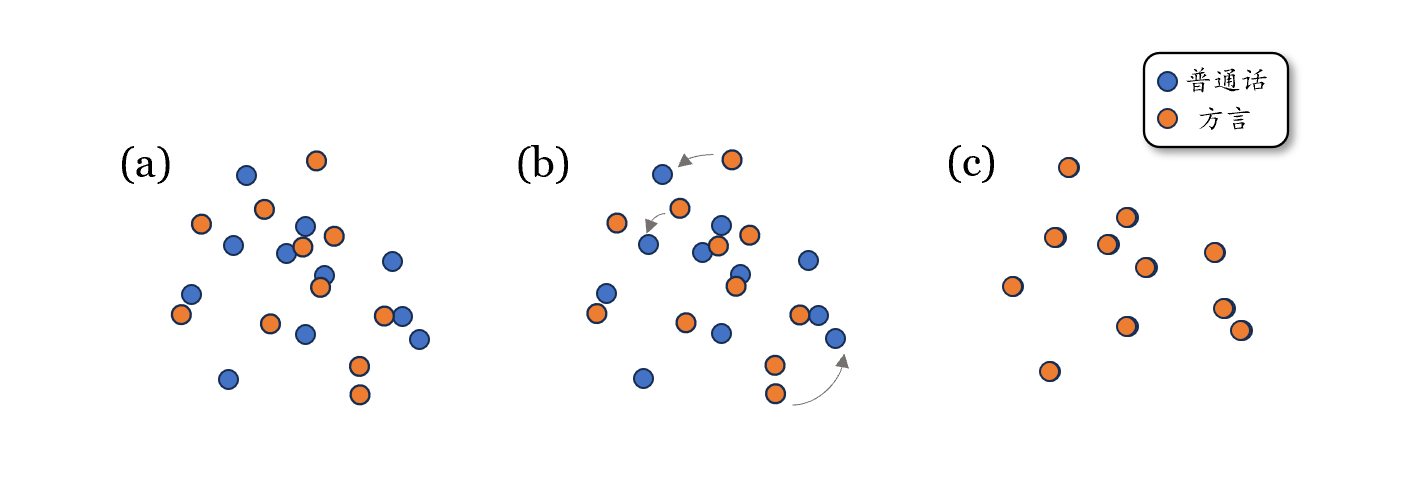
\includegraphics[scale=0.2]{Map.png}
    \end{figure}
\end{frame}
\begin{frame}
    为方便表示,定义运算符$\otimes$,称其为对一个矩阵$X$作元素层级上的函数矩阵操作$F$:
    \begin{equation}
        X \otimes F
    \end{equation}
    \begin{equation}
        X = \begin{bmatrix}
            x_{1,1} & x_{1,2} & \cdots & x_{1,N} \\
            x_{2,1} & x_{2,2} & \cdots & x_{2,N} \\
            \vdots & \vdots & \ddots & \vdots \\
            x_{L,1} & x_{L,2} & \cdots & x_{L,N}\\
        \end{bmatrix},F = \begin{bmatrix}
            f_{1,1} & f_{1,2} & \cdots & f_{1,N} \\
            f_{2,1} & f_{2,2} & \cdots & f_{2,N} \\
            \vdots & \vdots & \ddots & \vdots \\
            f_{L,1} & f_{L,2} & \cdots & f_{L,N}\\
        \end{bmatrix}
    \end{equation}
    \begin{equation}
        X \otimes F = \begin{bmatrix}
            f_{1,1}(x_{1,1}) & f_{1,2}(x_{1,2}) & \cdots & f_{1,N}(x_{1,N}) \\
            f_{2,1}(x_{2,1}) & f_{2,2}(x_{2,2}) & \cdots & f_{2,N}(x_{2,N}) \\
            \vdots & \vdots & \ddots & \vdots \\
            f_{L,1}(x_{L,1}) & f_{L,2}(x_{L,2}) & \cdots & f_{L,N}(x_{L,N})\\
        \end{bmatrix}
    \end{equation}
\end{frame}
\begin{frame}
    有特征矩阵$M_{\mathbb{D}}$和$M_{\mathbb{M}}$:
    \begin{equation}
        M_{\mathbb{D}} = \begin{bmatrix}
            d_{1,1} & d_{1,2} & \cdots & d_{1,N} \\
            d_{2,1} & d_{2,2} & \cdots & d_{2,N} \\
            \vdots & \vdots & \ddots & \vdots \\
            d_{L,1} & d_{L,2} & \cdots & d_{L,N}\\
        \end{bmatrix}
        M_{\mathbb{M}} = \begin{bmatrix}
            m_{1,1} & m_{1,2} & \cdots & m_{1,N} \\
            m_{2,1} & m_{2,2} & \cdots & m_{2,N} \\
            \vdots & \vdots & \ddots & \vdots \\
            m_{L,1} & m_{L,2} & \cdots & m_{L,N}\\
        \end{bmatrix}
    \end{equation}
    寻找函数矩阵F:
    \begin{equation}
        F = \begin{bmatrix}
            f_{1,1} & f_{1,2} & \cdots & f_{1,N}\\
            f_{2,1} & f_{2,2} & \cdots & f_{2,N}\\
            \vdots & \vdots & \ddots & \vdots \\
            f_{L,1} & f_{L,2} & \cdots & f_{L,N}
        \end{bmatrix}
    \end{equation}
    使得满足下式:
    \begin{equation}
        M_{\mathbb{D}} \otimes F = M_{\mathbb{M}} 
    \end{equation}
\end{frame}
\begin{frame}
    \begin{equation}
        M_{\mathbb{D}} \otimes F = M_{\mathbb{M}}
    \end{equation}
    即:
    \begin{equation}
        \begin{bmatrix}
            m_{1,1} & m_{1,2} & \cdots & m_{1,N} \\
            m_{2,1} & m_{2,2} & \cdots & m_{2,N} \\
            \vdots & \vdots & \ddots & \vdots \\
            m_{L,1} & m_{L,2} & \cdots & m_{L,N}
        \end{bmatrix}=\begin{bmatrix}
            f_{1,1}(d_{1,1}) & f_{1,2}(d_{1,2}) & \cdots & f_{1,N}(d_{1,N}) \\
            f_{2,1}(d_{2,1}) & f_{2,2}(d_{2,2}) & \cdots & f_{2,N}(d_{2,N}) \\
            \vdots & \vdots & \ddots & \vdots \\
            f_{L,1}(d_{L,1}) & f_{L,2}(d_{L,2}) & \cdots & f_{L,N}(d_{L,N})
        \end{bmatrix}
    \end{equation}
\end{frame}
\begin{frame}
    将映射关系限定为线性关系,则对矩阵中每个元素考虑线性回归:
    \begin{equation}
        \hat{y} = \beta_0 + \beta_1 x
    \end{equation}
    \begin{equation}
        \left\{ 
        \begin{aligned}
               \beta_1 &= \frac{\sum_{k=1}^{L} (\mathbf{V}_{{ij}_k}-\overline{\mathbf{V}_{ij}}) (\mathbf{U}_{{ij}_k}-\overline{\mathbf{U}_{ij}})}{\sum_{k=1}^{L} (\mathbf{V}_{{ij}_k}-\overline{\mathbf{V}_{ij}})^2}\\
            \beta_0 &= \overline{\mathbf{U}_{ij}}-\beta_1 \overline{\mathbf{V}_{ij}}
        \end{aligned}
        \right.
    \end{equation}
\end{frame}
\begin{frame}
    于是我们有线性映射关系矩阵,由映射关系权重矩阵$\Omega$和映射关系常数误差矩阵$E$构成。
    \begin{equation}
        \Omega = \begin{bmatrix}
            \omega_{1,1} & \omega_{1,2} & \cdots & \omega_{1,N}\\
            \omega_{2,1} & \omega_{2,2} & \cdots & \omega_{2,N}\\
            \vdots & \vdots & \ddots & \vdots \\
            \omega_{L,1} & \omega_{L,2} & \cdots & \omega_{L,N}
        \end{bmatrix},
        E = \begin{bmatrix}
            \varepsilon_{1,1} & \varepsilon_{1,2} & \cdots & \varepsilon_{1,N}\\
            \varepsilon_{2,1} & \varepsilon_{2,2} & \cdots & \varepsilon_{2,N}\\
            \vdots & \vdots & \ddots & \vdots \\
            \varepsilon_{L,1} & \varepsilon_{L,2} & \cdots & \varepsilon_{L,N}
        \end{bmatrix}
    \end{equation}
    $\Omega$和$E$即等价于映射函数矩阵$F$
    \begin{equation}
        F = \begin{bmatrix}
            f_{1,1} & f_{1,2} & \cdots & f_{1,N} \\
            f_{2,1} & f_{2,2} & \cdots & f_{2,N} \\
            \vdots & \vdots & \ddots & \vdots \\
            f_{L,1} & f_{L,2} & \cdots & f_{L,N}
        \end{bmatrix}
    \end{equation}其中
    \begin{equation}
        F_{i,j}(x) = \omega_{i,j} x + \varepsilon_{i,j}
    \end{equation}
\end{frame}
\section{结果与讨论}
\subsection{结果}
\begin{frame}{回归函数选择}
    考虑使用不同函数回归结果的均方根误差(RMSE),发现不同的常见函数的结果无明显差异。为避免过拟合,采用最简单的一元线性回归模型。
    \begin{figure}[h]
        \caption{\label{fig:regression}不同回归函数均方根误差矩阵热力图}
        \centering
        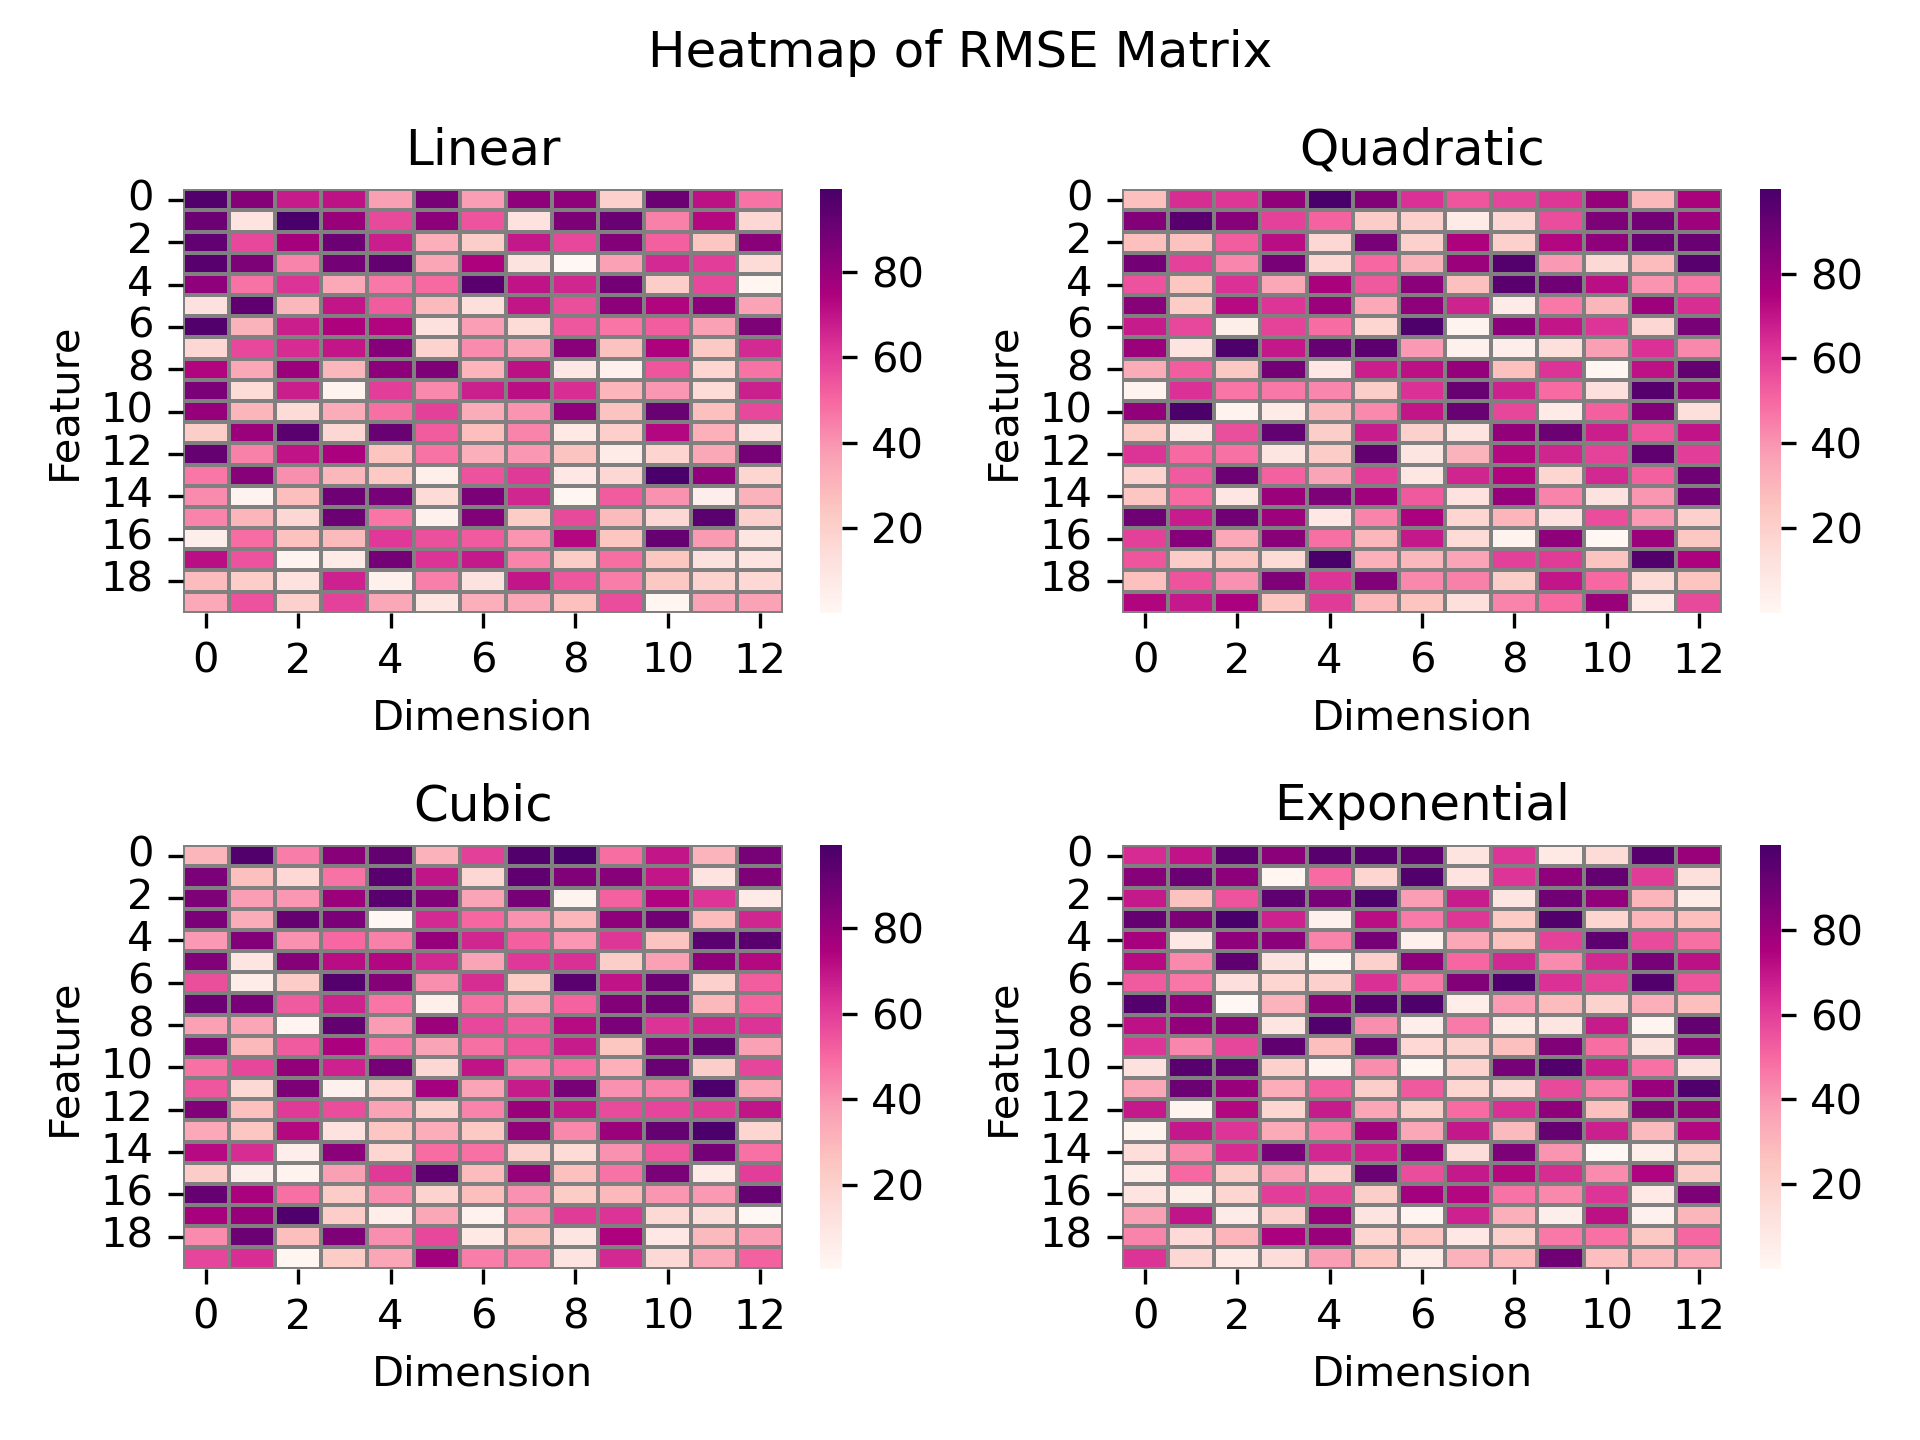
\includegraphics[scale=0.4]{RMatrix.png}
    \end{figure}
\end{frame}
\begin{frame}{映射关系矩阵}
    \begin{figure}[h]
        \caption{\label{fig:heatmap}映射关系矩阵热力图}
        \centering
        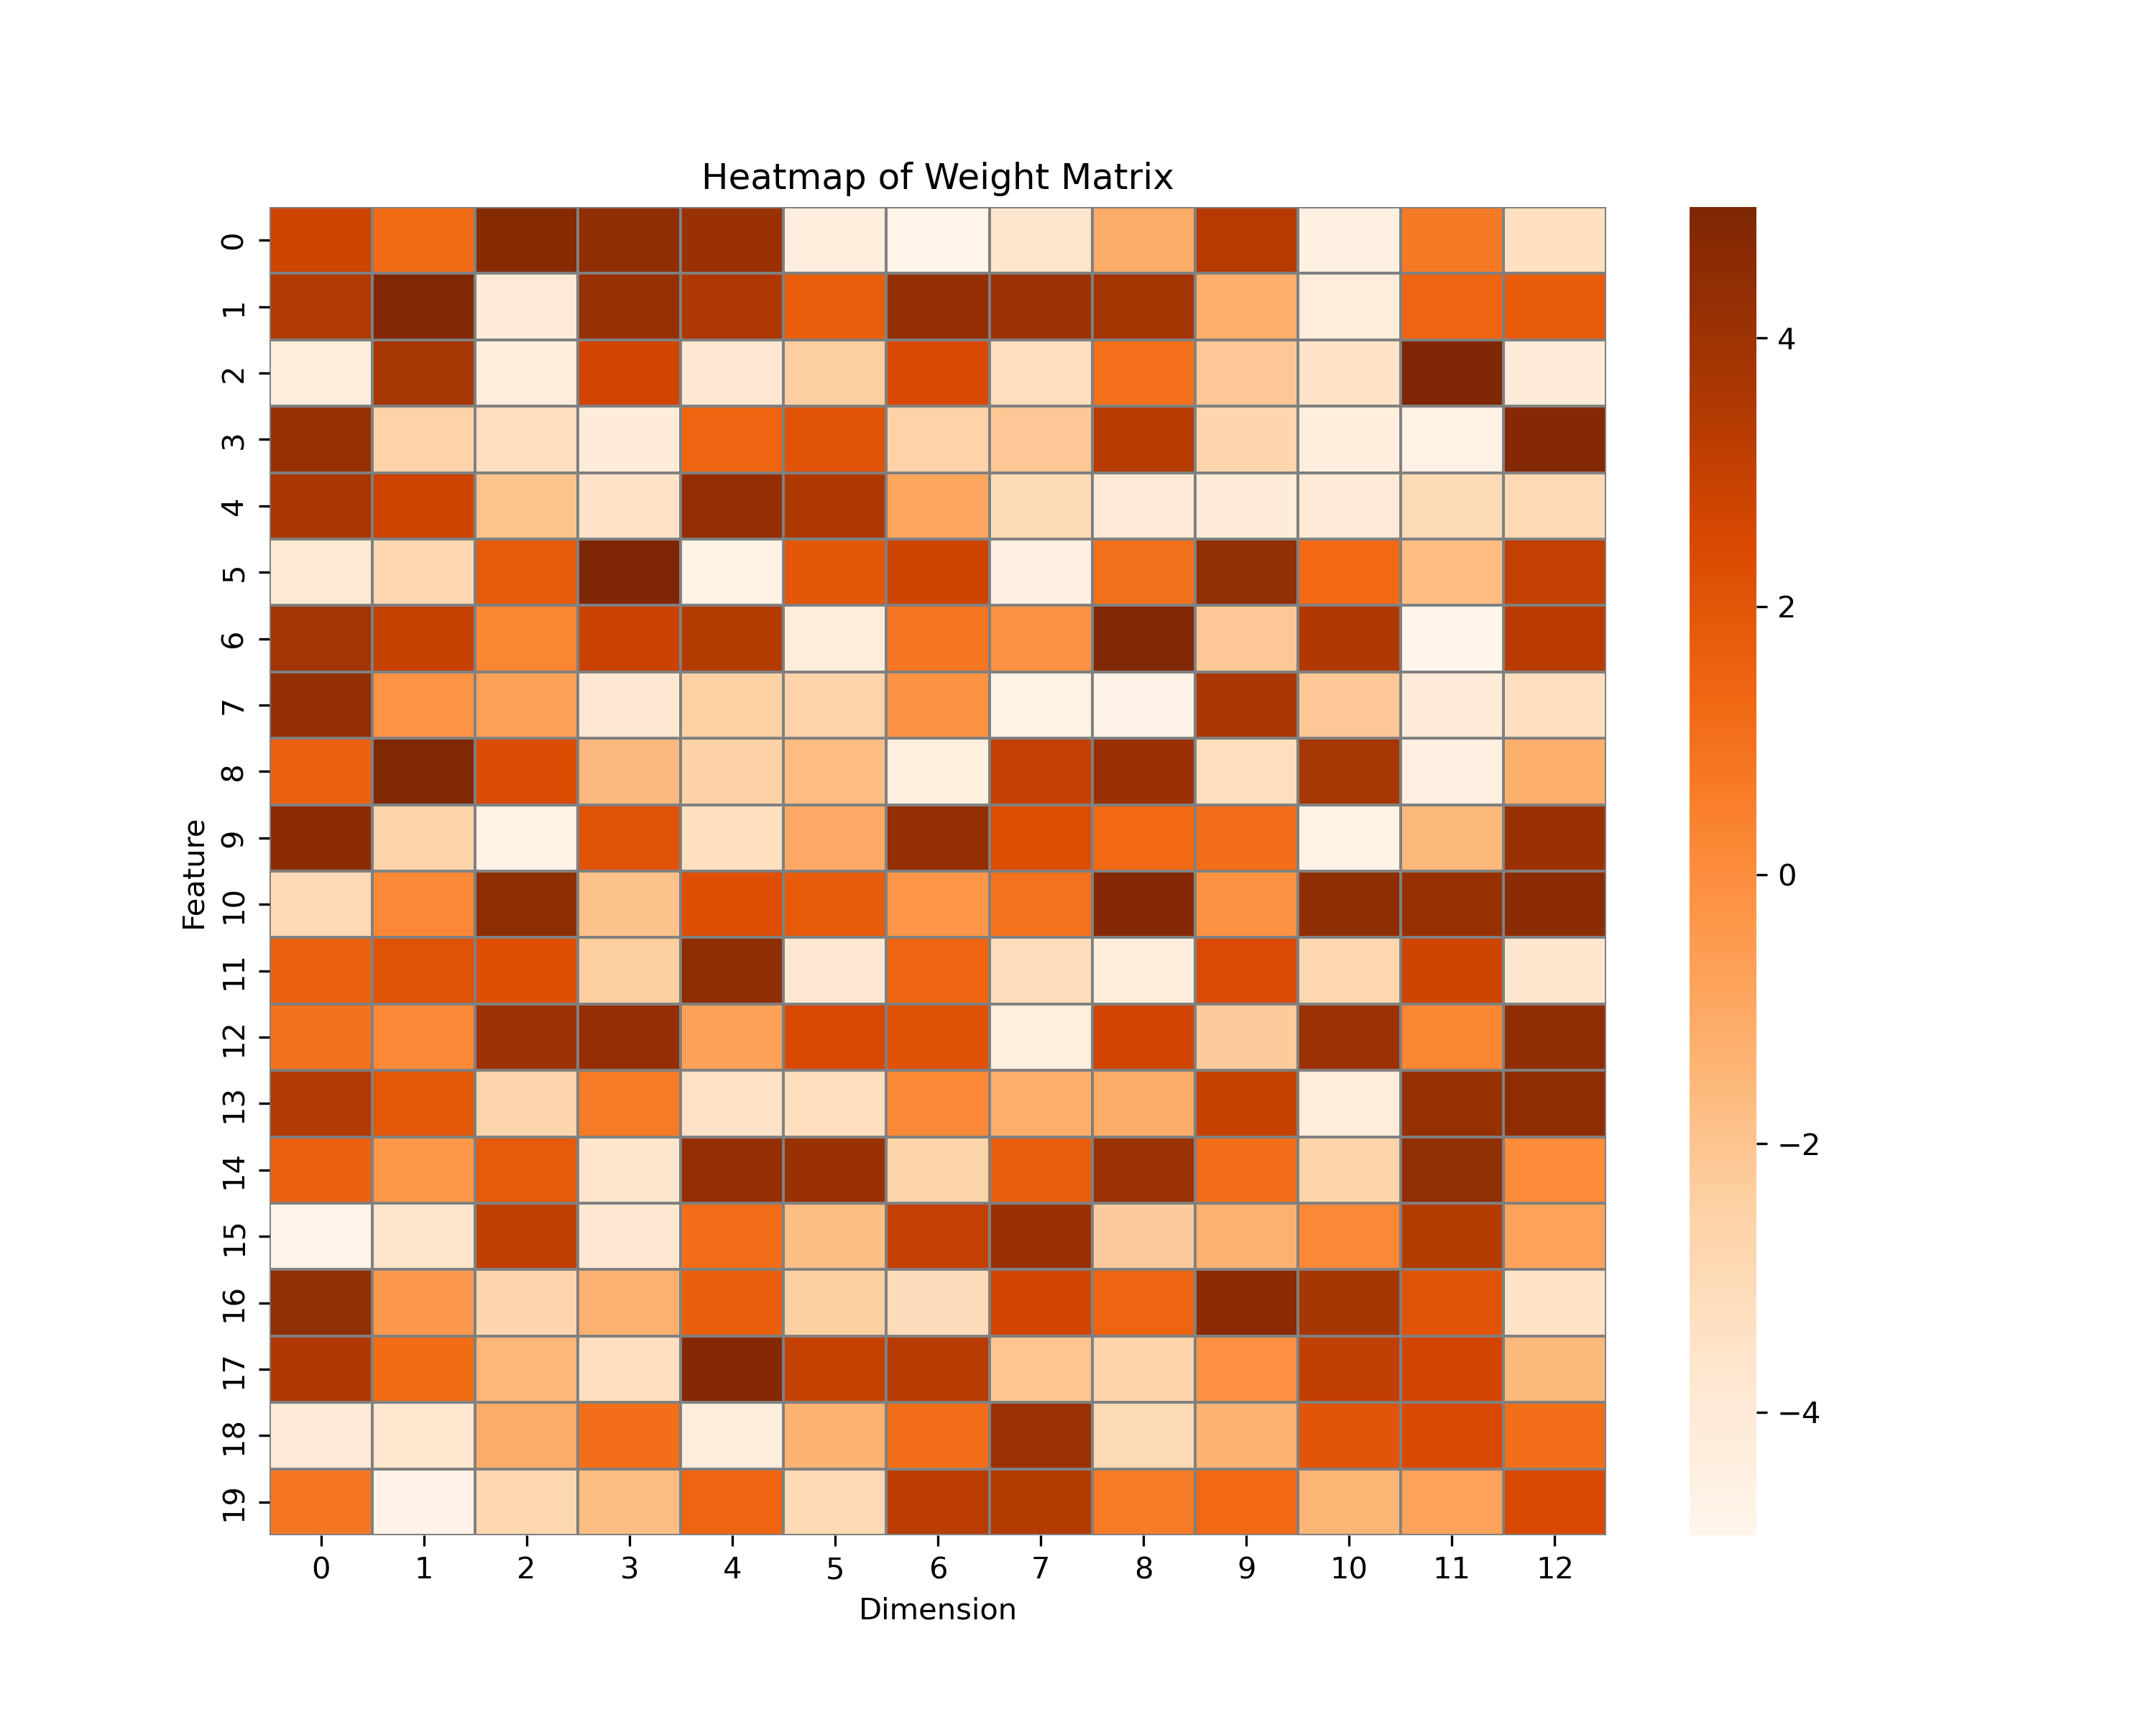
\includegraphics[scale=0.22]{Weight_Matrix_Heatmap.png}
        \hfill
        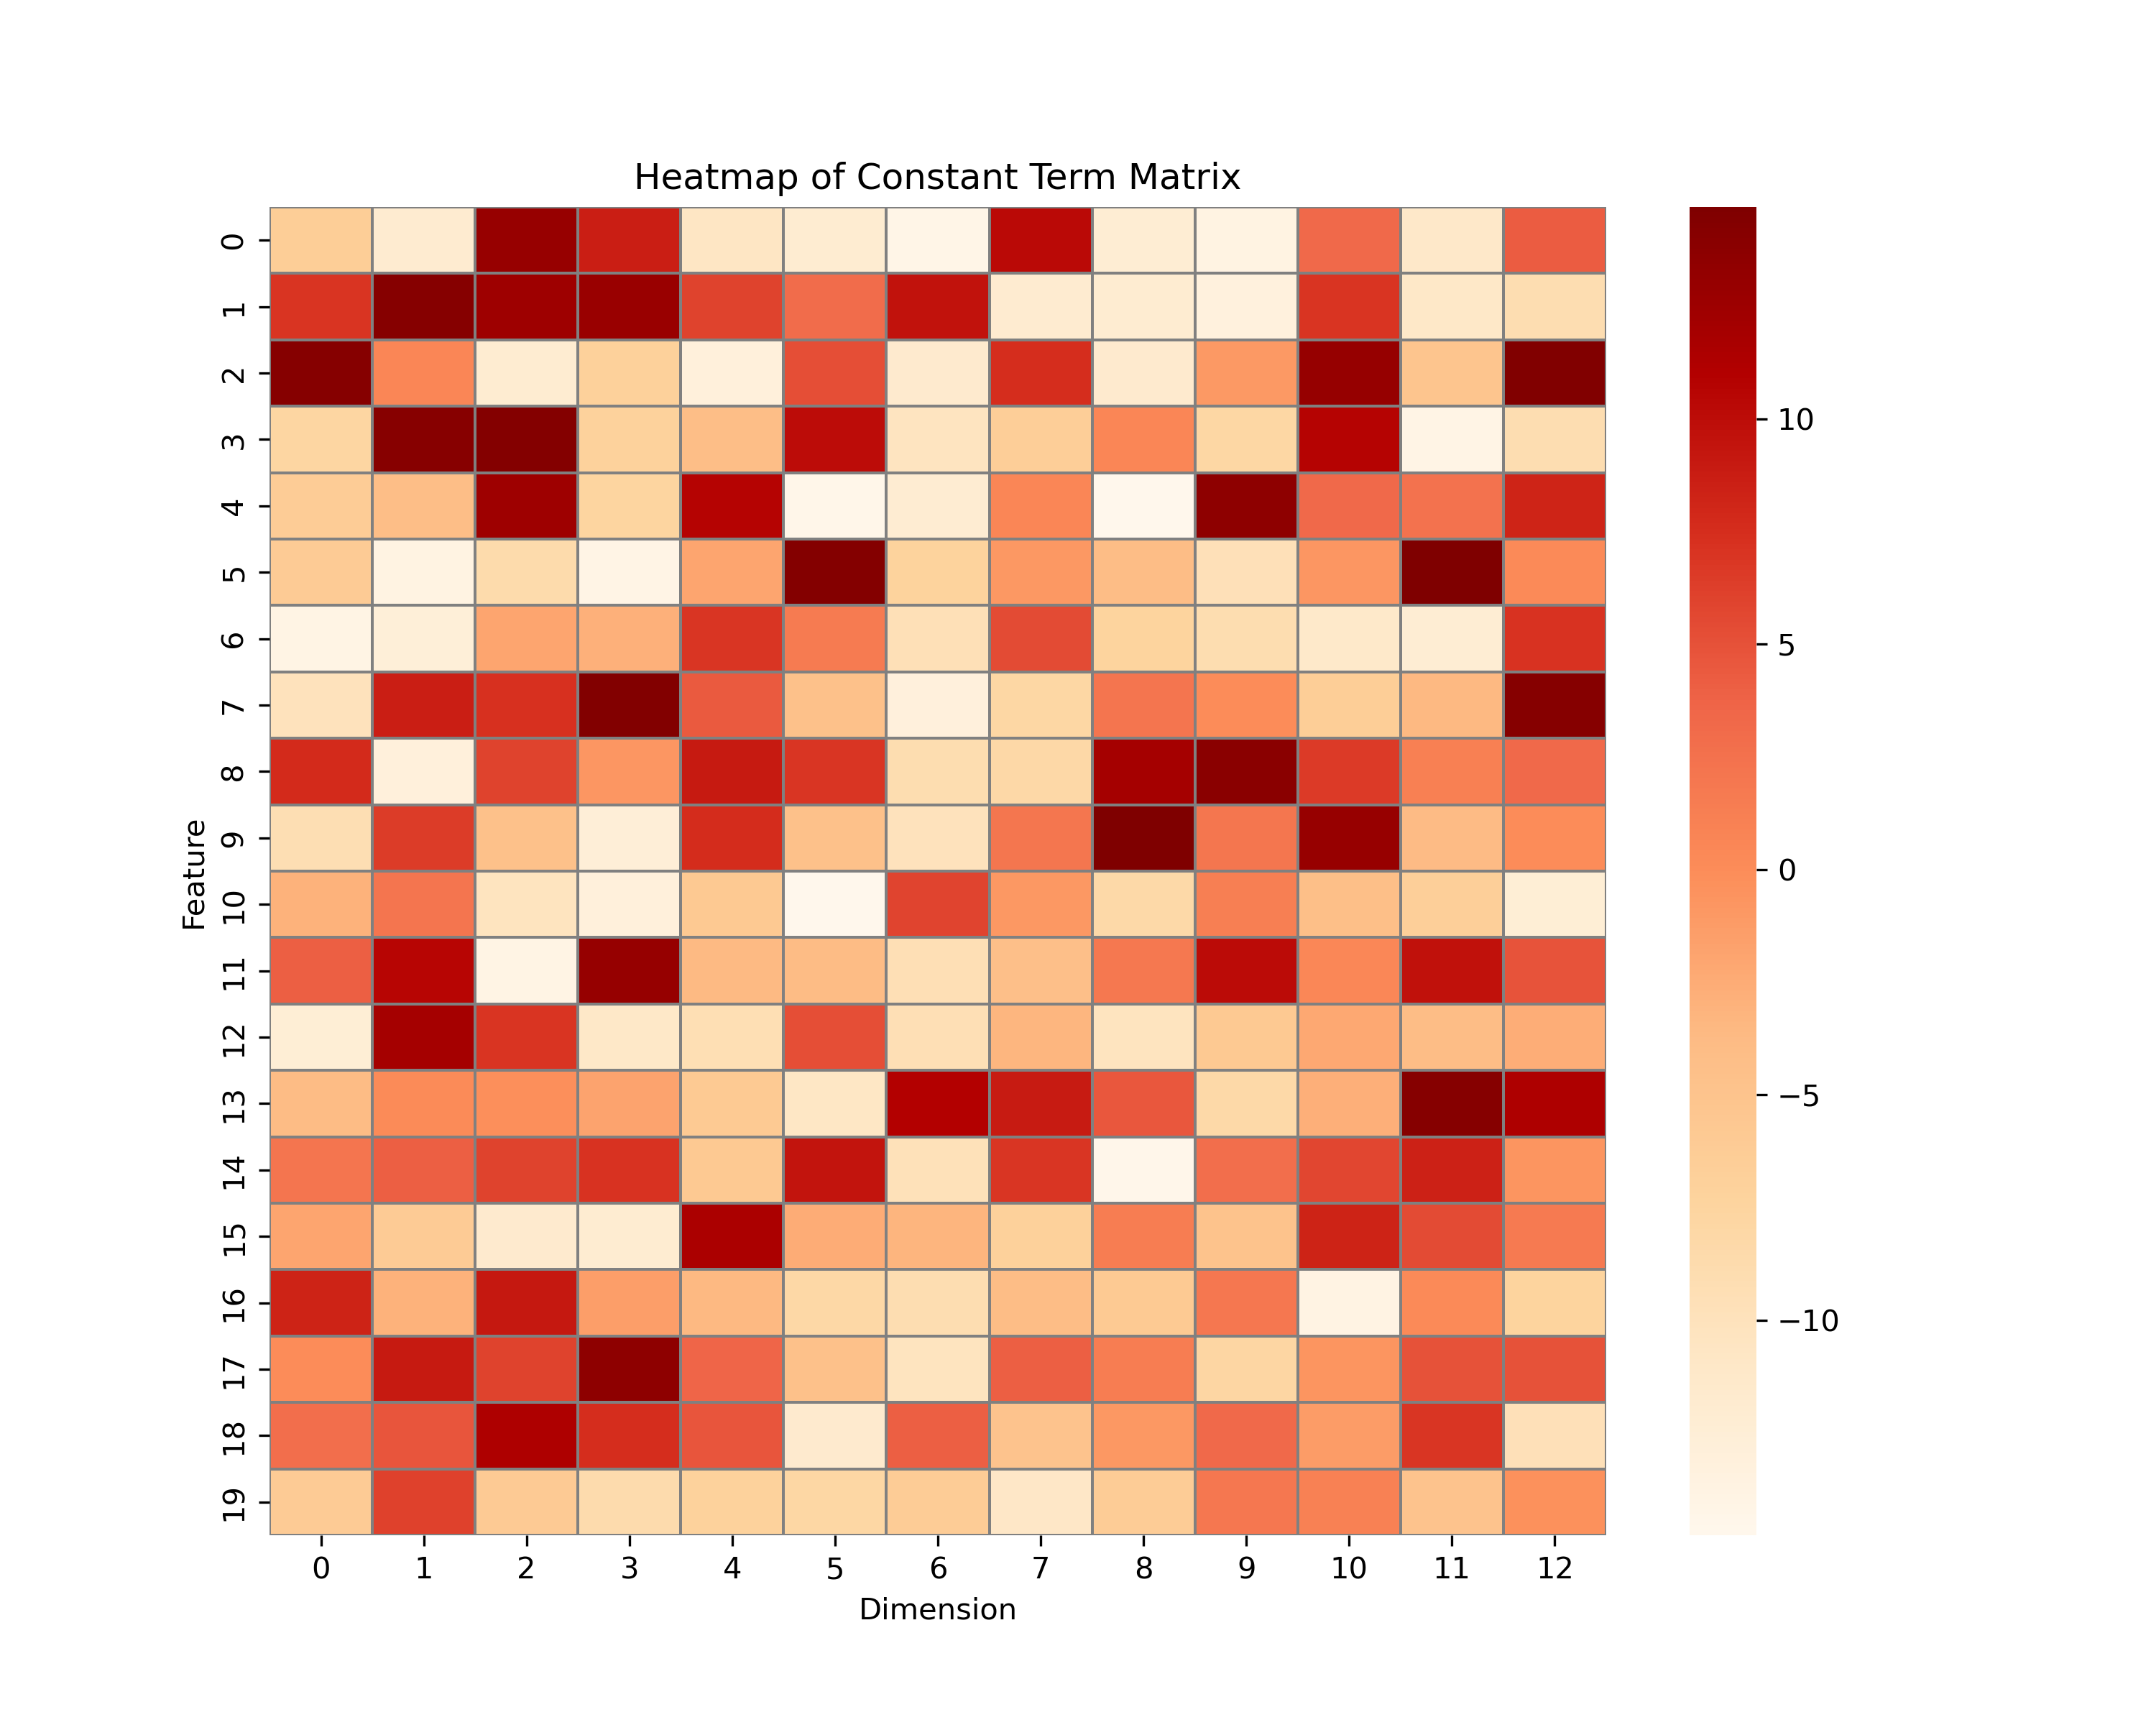
\includegraphics[scale=0.22]{Error_Matrix_Heatmap.png}
    \end{figure}
\end{frame}
\subsection{讨论}
\begin{frame}{讨论}
在本研究中,我们开发并验证了一个低成本普惠型智能家居方言指令转换器。以下是对研究结果的深入讨论:

\begin{itemize}
    \item 映射关系矩阵的有效性
    \item 回归函数的选择
\end{itemize}
\end{frame}
\begin{frame}{映射关系矩阵的有效性}
    \begin{itemize}
        \item \textbf{定义}: 将方言指令映射为标准普通话指令的关键组件。
        \item \textbf{重要性}: 决定转换器的准确性和用户体验。
    \end{itemize}
    
    \vspace{0.5cm}
    
    % Uncomment the following lines if you have a graph to insert
    % \begin{figure}
    %   \centering
    %   \includegraphics[width=0.7\linewidth]{accuracy_chart.png}
    %   \caption{映射关系矩阵的准确率}
    % \end{figure}
    
\end{frame}

\begin{frame}{影响因素分析与总结}
  \begin{itemize}
    \item \textbf{影响因素分析}:
    \begin{itemize}
      \item \textbf{数据覆盖率}: 广泛的方言样本提高了矩阵的适应性。
      \item \textbf{特征选择}: 使用MFCC和SVD特征提取增强了信号捕捉能力。
    \end{itemize}
    
    \vspace{0.5cm}
    
    \item \textbf{总结}:
    \begin{itemize}
      \item 映射关系矩阵表现优异,准确率高。
      \item 数据覆盖率和特征选择是关键因素。
      \item 实际应用中展示了良好的鲁棒性和稳定性。
    \end{itemize}
  \end{itemize}
\end{frame}
\begin{frame}
    通过对梅尔频率倒谱系数(MFCCs)的分析,我们构建了映射关系矩阵,包括映射关系权重矩阵 \( \Omega \) 和映射关系常数误差矩阵 \( E \)。实验结果表明,所提出的方法能够有效捕捉并转换方言指令,使得智能家居系统能够准确识别和执行相应的操作。然而,在不同方言之间,映射关系矩阵的准确性存在差异。这表明,不同方言的声学特征差异显著,未来可以通过进一步优化这些矩阵来提高对更多方言的识别精度。
\end{frame}
\begin{frame}{回归函数的选择}
    我们测试了多种回归函数,最终选择了一元线性回归模型。原因在于,在比较均方根误差(RMSE)后发现,复杂模型并未显著提高精度,反而增加了过拟合的风险。采用最简单的一元线性回归模型不仅能有效避免过拟合,还能保证模型的可解释性和计算效率。这种选择对低成本设备尤为重要,因为计算资源有限,简单模型在实际应用中更具可行性。
\end{frame}
\section{参考文献}
\subsection{参考文献}
\begin{frame}{参考文献}
    \bibliography{D:\\TaoLi\\Projects\\DialectTranslation\\Beamer\\references_beamer}
\end{frame}
\end{document}